\section{Evaluation}
\label{sec:msgt-evaluation}

In this section, we experimentally compare MSGT with SGT using our prototype in-memory DBMS. The evaluation focuses on 
two implementations: a graph-based scheduler (SGT) and a mixed graph-based scheduler (MSGT).

Experiments were performed using an Azure Standard D48v3 instance with 48 virtualized CPU cores and 192GB of memory. 
Prior to each experiment, tables are loaded, followed by a warm-up period, before a measurement period; both are of 
configurable length, we use 60 seconds and 5 minutes respectively. We measure the following metrics:
\begin{itemize}
\item \textbf{\emph{Throughput:}} number of transactions committed per second.
\item \textbf{\emph{Abort rate:}} rate at which transactions are being aborted.
\item \textbf{\emph{Average latency:}} the latency time of committed transactions (in $ms$) averaged across the 
measurement period.
\end{itemize}

Our experiments use the Yahoo! Cloud Serving Benchmark (YCSB)~\cite{DBLP:conf/cloud/CooperSTRS10}. YCSB was originally
designed to evaluate large-scale Internet applications, it is re-purposed here as a microbenchmark to allow various 
aspects of an OLTP workload to be altered. Specifically, we tweak the proportion of serializable transactions, differ 
the contention level, and increase the core count to measure scalability. YCSB has a one table with a primary key and 
10 additional columns each with 100B of random characters. For all our experiments, we use a YCSB table of 100K rows. 
There are two types of transaction: read or update, each contains 10 independent operations accessing 10  distinct 
items. Update transactions consist of 5 reads and 5 writes that  occur in random order. Read transactions consist 
solely of read operations. The proportion of update transactions is controlled by the parameter, $U$, it is fixed to 
50\% for our experiments. Data access follows a Zipfian distribution, where the frequency of access to hot records is 
tuned using a skew parameter, $\theta$. When $\theta = 0$, data is accessed with uniform frequency, and when 
$\theta = 0.9$ it is extremely skewed. In order to measure the impact of transactions running at weaker isolation we 
introduce an additional parameter, $\omega$, which controls the proportion of transactions running at 
\level{Serializable} isolation. The remainder are split between \level{Read Committed} (90\%) and 
\level{Read Uncommitted} (10\%).

\subsection{Isolation}
\label{sec:isolation}

\begin{figure}[htbp]
    \centering
    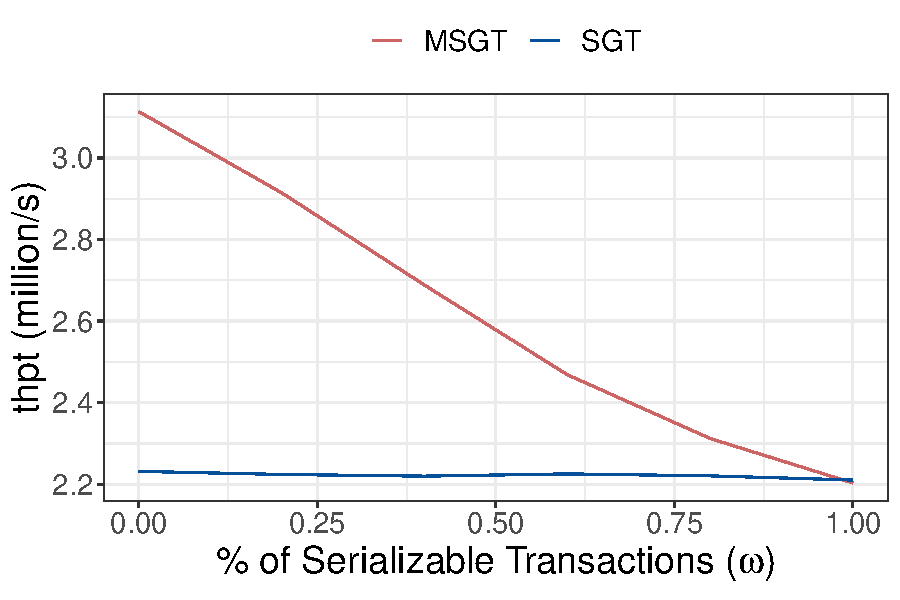
\includegraphics[width=0.6\linewidth]{figs/ycsb_isolation_thpt}%
    \caption{Throughput as serializable transactions ($\omega$) varied from 0\% to 100\%.}
    \label{fig:isolation-a}
\end{figure}




We begin with measuring the impact of increasing the proportion of transactions executing at \level{Serializable} 
isolation from 0\% to 100\%. This aims to test MSGT's ability to leverage its theoretical properties to offer increased 
performance when transactions are run at weaker isolation levels. For this experiment, we opt for a medium contention 
level, $\theta=0.8$, and the framework is configured to run with 40 cores.

In~\Cref{fig:isolation-a}, SGT's throughput is invariant 
to the proportion of \level{Serializable} transactions, 
this is anticipated as it is unable to take advantage of 
transactions' declared isolation levels, in effect, 
executing all transactions at \level{Serializable}. 
Meanwhile, the throughput of MSGT decreases as $\omega$ 
is increased, converging towards SGT's throughput. When 
there are no \level{Serializable} transactions 
($\omega = 0.0$), MSGT achieves a 39\% increase in 
throughput. At $\omega = 0.4$, this drops to a 21\%
increase and at $\omega = 0.8$ a 4\% gain is exhibited. 
When $\omega = 1.0$, SGT marginally outperforms MSGT, 
this can be attributed to the additional overhead of 
managing the MSG. This relationship is reflected in the
abort rate displayed in~\Cref{fig:isolation-b}, across 
the range of $\omega$, SGT's abort rate varies from a 3x 
increase over MSGT's abort rate to an equivalent abort 
rate when all transactions are executed at 
\level{Serializable}. A higher abort rate degrades the 
user experience, reduces throughput and, as can be seen
in~\Cref{fig:isolation-c}, harms latency.

\begin{figure}[htbp]
  \centering
  \subcaptionbox{Abort rate $vs.$ $\omega$\label{fig:isolation-b}}{%
    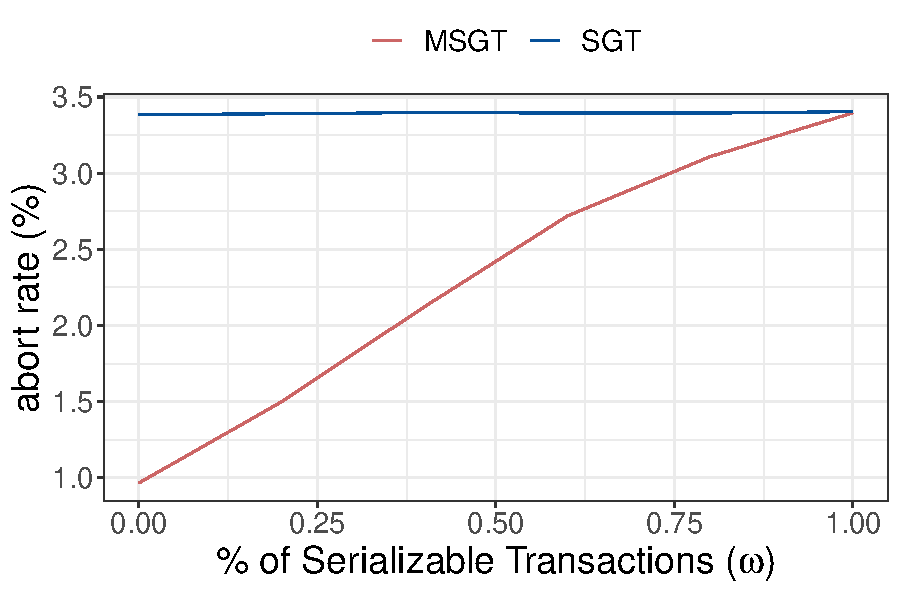
\includegraphics[width=0.49\linewidth]{figs/ycsb_isolation_abr}%
  }%
  \subcaptionbox{Average latency $vs.$ $\omega$.\label{fig:isolation-c}}{%
    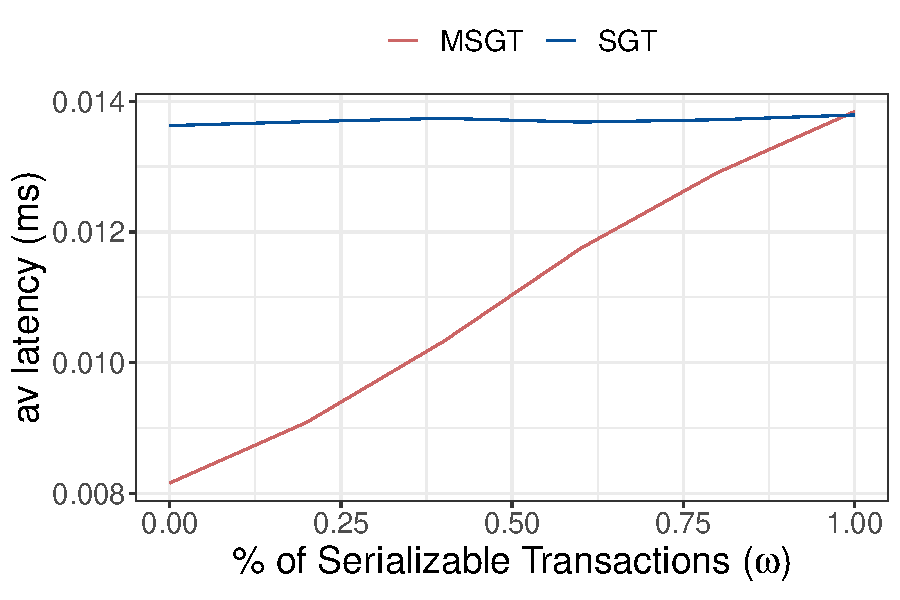
\includegraphics[width=0.49\linewidth]{figs/ycsb_isolation_lat}%
  }%
  \caption{Serializable transactions ($\omega$) varied from 0\% to 100\%.}
  \label{fig:isolation-exp}
\end{figure}


\subsection{Contention}
\label{sec:contention}

In the next experiment we measure the effect of increasing contention in the system by varying $\theta$ from 
0.6 to 0.9. Contention happens when multiple transactions try to read or write the same database item. In 
theory, contention increases the chance of conflicts between transactions. This should translate into an 
increase in the number of edges inserted into the conflict graph. Under SGT all edges are inserted, whereas, 
MSGT utilizes isolation levels to be more selective over edge insertions (only adding relevant or obligatory 
edges) hence it inserts less edges into the conflict graph, and should find less cycles (aborts) compared to SGT. We 
set the proportion of \level{Serializable} transactions to $\omega=0.2$. Again the experiment was run with 40 cores.

\begin{figure}[htbp]
    \centering
    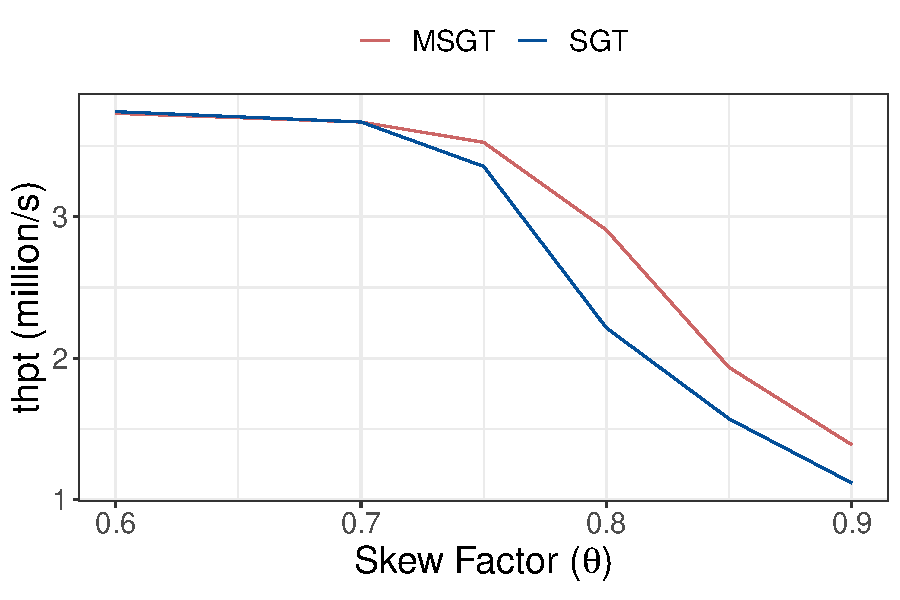
\includegraphics[width=0.6\linewidth]{figs/ycsb_contention_thpt}%
      \caption{Throughput as contention factor ($\theta$) varied from 0.6 to 0.9.}
    \label{fig:contention-a}
\end{figure}

\begin{figure}[htbp]
  \centering
  \subcaptionbox{Abort rate $vs.$ $\theta$\label{fig:contention-b}}{%
    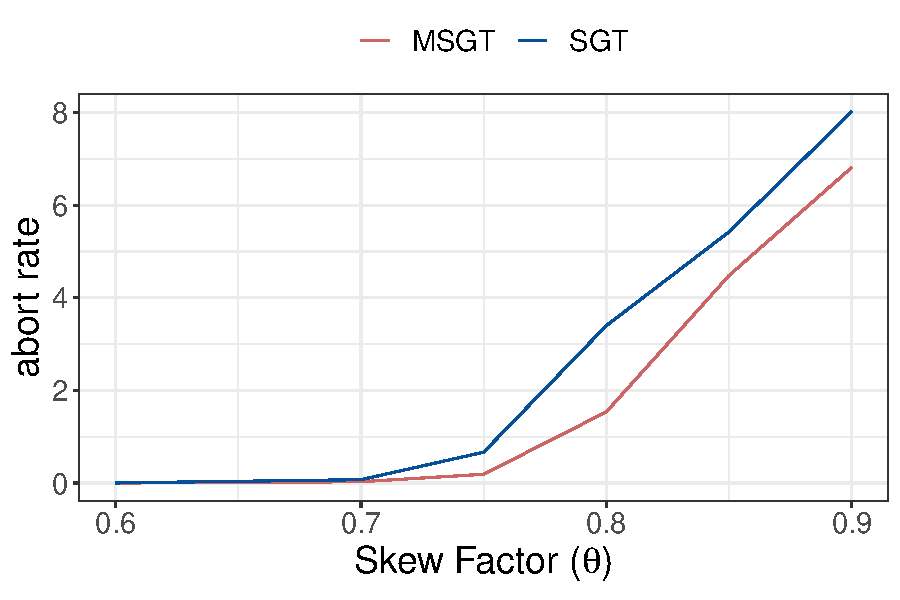
\includegraphics[width=0.49\linewidth]{figs/ycsb_contention_abr}%
  }%
  \subcaptionbox{Average latency $vs.$ $\theta$.\label{fig:contention-c}}{%
    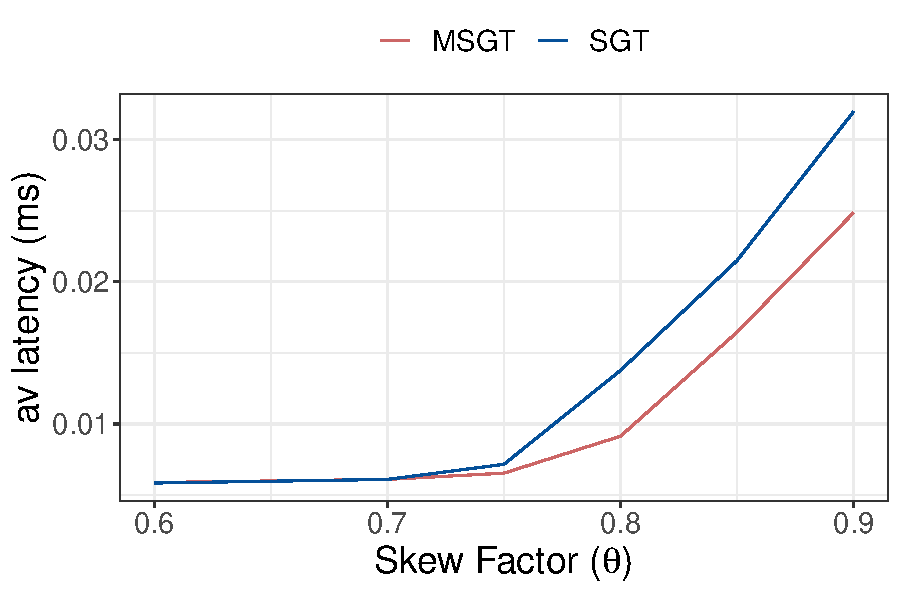
\includegraphics[width=0.49\linewidth]{figs/ycsb_contention_lat}%
  }%
  \caption{Contention factor ($\theta$) varied from 0.6 to 0.9.}
  \label{fig:contention-exp}
\end{figure}


\Cref{fig:contention-a} displays the throughput 
of SGT and MSGT as the contention is increased. 
As $\theta$ increases the throughput decreases
for both protocols. For low levels of contention
SGT performs marginally better than MSGT ($<$1\% 
difference), but under high contention this reverses 
and MSGT offers a 24\% increase in throughput.
\Cref{fig:contention-b} shows that after $\theta = 0.7$, 
the abort rate begins increasing for both protocols. 
At the highest level of contention ($\theta = 0.9$), 
0.1\% of the data is accessed by 35\% of the queries, 
and SGT aborts 17\% more transactions than MSGT. Lastly, 
in~\Cref{fig:contention-c}, above $\theta = 0.7$, MSGT 
achieves between a 9\% and 28\% reduction in the average 
latency.

\subsection{Update Rate}
\label{sec:update-rate}

For the next experiment, we explore the effect of 
varying the proportion of update operations ($U$) within 
each transaction. For this experiment, we opt for a
medium contention level, $\theta = 0.8$, set the 
proportion of \level{Serializable} transactions to $\omega = 0.2$, with the framework configured to run with 40 cores. 

From~\Cref{fig:update-rate-a} it can be seen that at 
both extremes $U=0.0$ and $U=1.0$ MSGT displays no 
benefit over SGT. When $U=0.0$, the workload is 
read-only thus no (\textsf{ww}, \textsf{wr}, 
\textsf{rw}) conflicts are generated. Conversely, with 
$U=1.0$ all transactions are write-only, hence only 
\textsf{ww} conflicts can occur, which are always inserted
into the graph under SGT and MSGT. In both cases MSGT is 
unable leverage its selective conflict detection rules.
However, between the extremities MSGT is able to produce 
higher throughput compared to SGT (up to 28\% when $U=0.2$).

\begin{figure}[htbp]
    \centering
    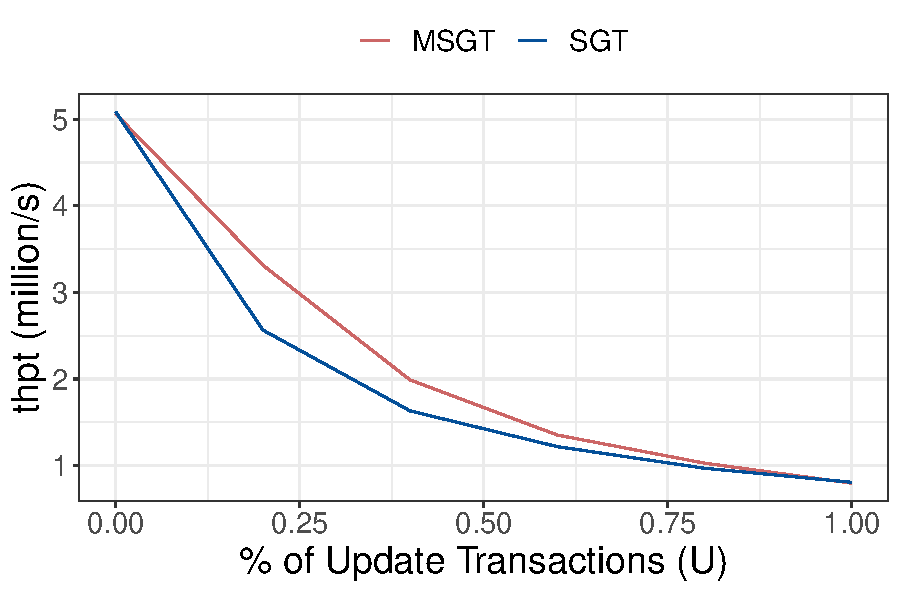
\includegraphics[width=0.6\linewidth]{figs/ycsb_update_rate_thpt.pdf}%
    \caption{Throughput as update rate transactions ($U$) varied from 0.0 to 1.0.}
    \label{fig:update-rate-a}
\end{figure}



\subsection{Scalability}
\label{sec:scalability}

In this experiment we fix the workload factors and vary 
the core count (1 to 40) to evaluate MSGT's scalability 
compared to SGT. We anticipate that MSGT scales better 
than SGT as its scheduler generally performs less work 
(edge insertions and cycle checking). 
From~\Cref{fig:scalability-a} it can be seen that until 
20 cores the throughput of both protocols is 
indistinguishable; in fact, up to 10 cores SGT exhibits 
between a 1.2\% and 3.1\% increase over MSGT. After this 
point, a gap appears, at 30 cores MSGT has 13.1\% higher 
throughput and at 40 cores this difference increases to 
27.9\%. 

In~\Cref{fig:scalability-b} it can be seen the abort 
rate of the protocols starts to diverge after 10 
cores: SGT has an abort rate of 1.65\% and 3.39\% at 30 
and 40 cores respectively, whereas, MSGT's is 0.50\% and 
1.54\%.

\begin{figure}[htbp]
  \centering
 \subcaptionbox{Throughput $vs.$ cores.\label{fig:scalability-a}}{%
    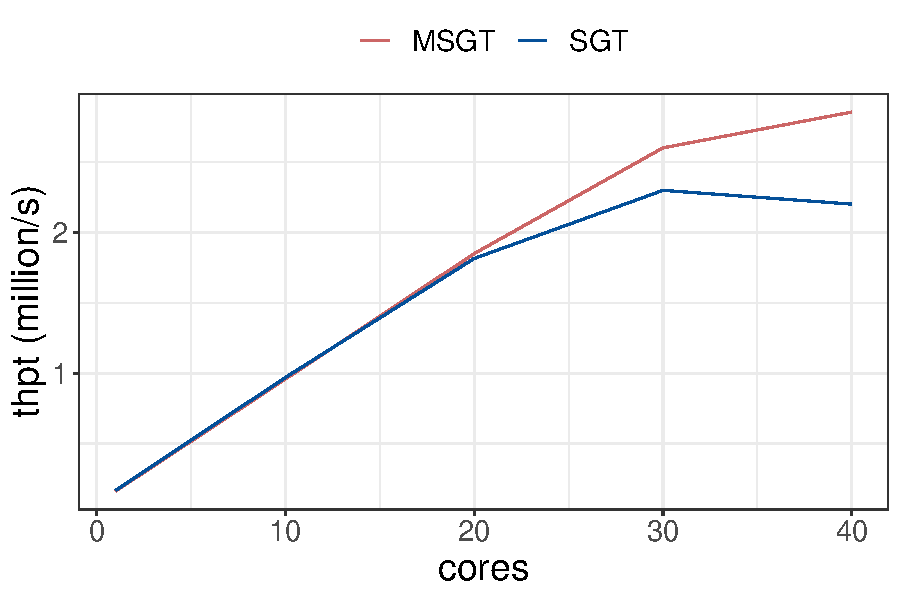
\includegraphics[width=0.49\linewidth]{figs/ycsb_scalability_thpt}%
  }%
  \subcaptionbox{Abort rate $vs.$ cores.\label{fig:scalability-b}}{%
    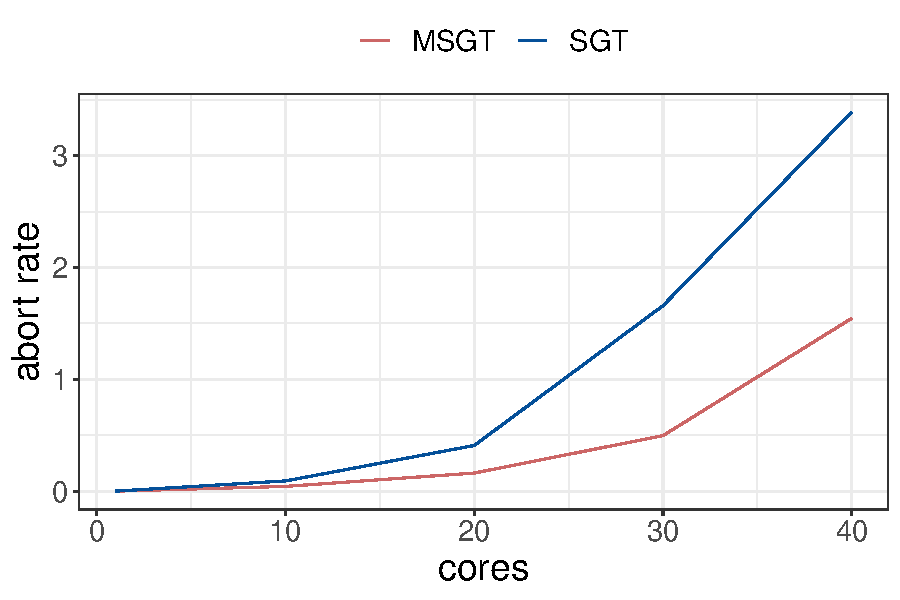
\includegraphics[width=0.49\linewidth]{figs/ycsb_scalability_abr}%
  }%
  \caption{Core count varied 1 to 40.}
  \label{fig:scalability-exp}
\end{figure}


